% das Papierformat zuerst
%
%\documentclass[a4paper, 11pt,bibtotoc]{scrartcl}
\documentclass[a4paper, 11pt,bibtotoc,abstracton]{scrreprt}  

%Für URL
\usepackage{url}
\renewcommand{\UrlFont}{\rmfamily}

%Für Zitaten
\usepackage{cite}

%Abkürzungen
\usepackage{acronym}


%Inhaltsverzeichnis bearbeiten
\usepackage{tocbibind}

% für mathematische Symbole
\usepackage{amsmath}


% Vektorgrafiken mit Latex importieren
\usepackage{import}

\usepackage[colorlinks=false, pdfborder={0 0 0}]{hyperref}
%documentclass[a4paper, 12pt]{article}  
% deutsche Silbentrennung
\usepackage[german,english]{babel}
\renewcommand{\sectfont}{\rmfamily\bfseries}
% wegen deutschen Umlauten
\usepackage[utf8]{inputenc}
\usepackage{graphicx}
\usepackage{subfigure}\hyphenation{Bit-rate}

%Algorithm schreiben
\usepackage{algorithm2e}

%Tabellen
\usepackage{booktabs}
\usepackage{multirow}
\usepackage{colortbl}
\usepackage{wrapfig}

%Farben
\usepackage{color}
\usepackage{listings}%Code einbinden
\definecolor{darkblue}{rgb}{.08,.21,.36}
\definecolor{darkred}{rgb}{.6,.19,.20}
\definecolor{darkgreen}{rgb}{0,.6,0}
\definecolor{red}{rgb}{.98,0,0}
\definecolor{lightblue}{rgb}{0.8,0.85,1}
%\definecolor{lightgrey}{rgb}{0.98,0.98,0.98}
\definecolor{lightgrey}{gray}{.98}
\definecolor{black}{rgb}{0.0,0.0,0.0}


\lstloadlanguages{C++}
\lstset{%
  language=C++,
  basicstyle=\small,
  commentstyle=\itshape\color{darkgreen},
  keywordstyle=\bfseries\color{darkblue},
  stringstyle=\color{darkred},
  showspaces=false,
  showtabs=false,
  columns=fixed,
  backgroundcolor=\color{lightgrey},
  numbers=left,
  frame=single,
  numberstyle=\tiny,
  breaklines=true,
  showstringspaces=false,
  xleftmargin=1cm,
  basicstyle=\small
}%

\usepackage{amssymb}%Mathematische Symbole, wie R,N,Q,Z,...
\setlength{\parindent}{0pt} %einrücken nach absatz verhindern
%\usepackage{setspace}%Zeilenabstand
\usepackage{algorithmic}%Für Pseudocode

%%%%%%%%%%%%%%%%%%%%%%%%%%%%%%%%%%%
%Seiten Kopf- und Fußzeilen
\usepackage[automark,						
		headsepline,								
		plainfootsepline, 
		]{scrlayer-scrpage}

\automark[section]{chapter} 
\pagestyle{scrheadings}			

\clearscrheadings	%Alte Kopfformatierungen entfernen
\clearscrplain		%Alte Plain-Formatierung entfernen
\clearscrheadfoot %Alten Fuß entfernen
\cfoot[\pagemark]{\pagemark}%Seitenzahl zentriert im Fuß 
\ihead{\leftmark}
\ohead{\rightmark} 
 
%%%%%%%%%%%%%%%%%%%%%%%%%%%%%%%%%%%

\begin{document}
\begin{titlepage}
\begin{center}
{\huge \textbf{Philipps-Universität Marburg}}\\[0.5cm]
\textbf{Fachbereich 12 - Mathematik und Informatik}\\[0.5cm]

\begin{figure}[h]
	\centering
		
\includegraphics[width=0.8\textwidth]{fig/unilogo.pdf}
\end{figure}

{\huge \textbf{{\large \\[1cm]Master Thesis}}}
\\[1cm]

{\Huge \textbf{Dynamic Insertion of 3D Objects\\ from CAD Files into Unreal Engine}}
\\[1cm]

{\large  Matija Mišković}\\
{\large September 2022}\\[3cm]

{\large
Supervisor:\\ Prof. Dr. Thorsten Thormählen\\[1cm]
Research Group Graphics and Multimedia Programming}

\end{center}
\end{titlepage}
\newpage
\thispagestyle{empty}
\section*{}
\newpage
\thispagestyle{empty}
\vspace*{7cm}
\textbf{\Large {Declaration of Originality}}\\[0.5cm]
I,  Matija Mišković (Computer Science Student at Philipps-University Marburg, Student-ID:
3139015), confirm that the submitted thesis is original work and was written by me without further assistance. Appropriate credit has been given where reference has been made to the work of others.
The thesis was not examined before, nor has it been published. The submitted electronic version of
the thesis matches the printed version.\\[1cm]
Marburg, 29. September 2022\\[0.5cm]
 Matija Mišković
\newpage
\shipout\null

%\setstretch {1.15}%Zeilenabstand setzen

  
% hier beginnt das Dokument

\begin{abstract}
Unreal Engine is a popular video game development engine which in recent years has gained a lot of popularity in various different fields for all of the functionalities and features it offers. However, those are not enough to fulfil all the new requirements expected from it, especially as some would generally not be used in game development. One such feature is importing and creating new 3D objects from CAD files during the runtime of an Unreal program. In this thesis it will be demonstrated how this can be achieved and how users can interact with these new objects. For these purposes a plug-in for Unreal Engine and a standalone, interactive program were developed.
\end{abstract}
 
\newpage\thispagestyle{empty}\hspace{1em}\newpage

\begin{otherlanguage}{german}
\begin{abstract}
Die Unreal Engine ist eine beliebte Engine für die Entwicklung von Videospielen, die in den letzten Jahren aufgrund ihrer zahlreichen Funktionen und Merkmalen in verschiedenen Bereichen sehr beliebt geworden ist. Diese reichen jedoch nicht aus, um alle neuen Anforderungen zu erfüllen, die an sie gestellt werden. Zumal da einige davon in der Regel nicht für die Spieleentwicklung verwendet werden. Ein solches Feature ist das Importieren und Erstellen neuer 3D-Objekte aus CAD-Dateien während der Laufzeit eines Unreal-Programms. In dieser Arbeit soll gezeigt werden, wie dies erreicht werden kann und wie der Benutzer mit diesen neuen Objekten interagieren kann. Zu diesem Zweck wurden ein Plug-in für die Unreal Engine und ein eigenständiges, interaktives Programm entwickelt.
\end{abstract}
\end{otherlanguage} 

\newpage\thispagestyle{empty}\hspace{1em}\newpage
\pagenumbering{Roman}
\setcounter{page}{1}
\renewcommand{\contentsname}{Table of Contents}
\tableofcontents
\newpage
\newpage\thispagestyle{empty}\hspace{1em}\newpage
\pagenumbering{arabic}
\setcounter{page}{1}
\chapter{Introduction}
The topic of this thesis is the dynamic insertion of 3D objects, defined in computer-aided design (\acs{CAD}) files, into an Unreal Engine program while it is running. Especially important for the project is why this might even be a problem and how it can actually be realized. For these purposes an Unreal Engine plug-in was developed which enables such a functionality and an additional Unreal Engine program which implements the plug-in and can be used to present and interact with the objects in a multi-user desktop or virtual reality environment.

%%%%%%%%%%%%%%%%%%%%%%%%%%%%%%%%%%%%%%%%%%%%%%%%%%%%%%%%%%%%%%%%%%%%%%%%%%%%%%%%%%%
\section{Motivation}

Virtual reality (\acs{VR}) is a relatively new field which is constantly seeing a lot of interest and innovation for all the new possibilities it opens up in software development and user interaction. In recent years \acs{VR} has been used in many companies in various industries such as engineering, architecture and healthcare and this number keeps on growing\cite{bib:VRFields}. One such company is Inosoft.\\
Inosoft is a software development firm in Marburg which was founded in 1993 and has since worked and consulted over two thousand projects for various companies including Viessmann, CSL Behring, Sanofi and many more \cite{bib:InosoftAbout}. They are also interested in \acs{VR} and have been working in the field since 2016. Inosoft was interested in establishing a working relationship with the Phillips University Marburg. As such they reached out with some projects in the field of \acs{VR}. Among them was designing and developing a concept to dynamically insert and interact with objects from \acs{CAD} files in a running Unreal Engine environment.\\
There are definitely certain scenarios where this could be a very useful tool. As an example, let us take a software Inosoft developed which is used to train workers in a digital production plan while the physical building was being built\cite{bib:InosoftProject}. The employees could put on a VR headset and find themself in a digital replica of the building. There they could simulate and test their workflow in order to find possible inefficiencies. This tool significantly reduced the time needed to train employees. Slight problems arise when things about the model need to be added or changed. First the changes need to be implemented in Unreal, packaged for standalone use and then redistributed to everyone who needs to use them. It would be a lot simpler if the program could simply open a file and add new objects without ever having to change the version of it.\\
Another use-case where this could be useful is in collaborative design or presenting 3D models. Instead of having to make the scene and import everything beforehand and distribute this version of the program, simply having a program that can open a file and have the model appear for everyone involved could save a lot of time and effort.\\
So, seeing as there are uses for this technology it makes sense to look into how it could be done and what the limitations are, as well as looking into why this isn't already officially part of Unreal Engine.

%%%%%%%%%%%%%%%%%%%%%%%%%%%%%%%%%%%%%%%%%%%%%%%%%%%%%%%%%%%%%%%%%%%%%%%%%%%%%%%%%%%
\section{Goals}\label{chp:Goals}   
The main goal of this work is to develop an efficient and user-friendly plug-in which will make it possible to load 3D objects from the most common \acs{CAD} formats during the runtime of an Unreal Engine program. Additionally, another software will be developed to use the plug-in and allow simple interactions with these objects in a normal desktop window as well as in a virtual reality environment.

%%%%%%%%%%%%%
\subsubsection{Efficiency} 
The developed plug-in should be capable of handling large amounts of data seeing as the models which can be found in \acs{CAD} files can be incredibly large, containing thousands or millions of vertices and polygons. If the plug-in were to affect the runtime performance in a significant way, such as causing stutters or freezing the program all together, it would severely worsen the user experience and invalidate the whole point of the program.

%%%%%%%%%%%%%
\subsubsection{Expandability} 
The field of computer-aided design is very wide and there are countless programs and formats for all the varying use-cases in which it is being used. That is why creating one solution for all of those is complicated and out of the scope and possibilities of this project. Instead, it is preferable to concentrate on creating a simple to use and understand system which can then be further improved upon and adjusted for the concrete cases of clients or projects.

%%%%%%%%%%%%%%%%%%%%%%%%%%%%%%%%%%%%%%%%%%%%%%%%%%%%%%%%%%%%%%%%%%%%%%%%%%%%%%%%%%%
\section{Thesis Structure}
In Chapter \ref{chp:UnrealEngine} the Unreal Engine will be clarified and explained. Seeing as this is both the tool which is being used for development as well as being the software for which the plug-in is being developed, an understanding of how it works and what its limitations are is needed in order to better grasp the project and what problems might arise. It is a rather expansive tool so not everything will be covered, only the more basic aspects and the concrete parts which play a role for this project. Then, in Chapter \ref{chp:ObjectLoading}, the plug-in will be analysed, starting off with how the files are parsed and into what sort of form they are transformed in order to be used. After that comes the actual mesh generation, how it is achieved and where extra attention is required. In Chapter \ref{chp:ObjectInteraction} it will be illustrated in what ways users can interact with the newly created objects, either using mouse and keyboard or virtual reality equipment. In Chapter \ref{chp:Results} the developed programs will be presented, evaluated and compared to similar software to see where its strengths and weaknesses are. Lastly in Chapter \ref{chp:Conclusion} the accomplished goals and some possible further projects and improvements will be discussed.

%%%%%%%%%%%%%%%%%%%%%%%%%%%%%%%%%%%%%%%%%%%%%%%%%%%%%%%%%%%%%%%%%%%%%%%%%%%%%%%%%%%
\section{Related Works}

When it comes to this topic there are unfortunately not that many similar works. Generally for importing \acs{CAD} files into the Unreal Engine editor, Datasmith definitely needs to be mentioned. Datasmith is an official set of tools and plug-ins created by Epic Games, the developers of Unreal Engine, to simplify and streamline the process of importing various \acs{CAD} formats into the engine\cite{bib:DSDoc}. It is important to note that the main focus of Datasmith is to make the process of transferring a model from a \acs{CAD} software into the Unreal Engine editor smoother and more efficient during development. Nonetheless amongst the many features it has it does also contain a plug-in for loading the models in runtime\cite{bib:DSRunDoc}. This plug-in was initially released in August 2021 and is still being developed. Even upon installation there are clear warnings that the software is still in beta. There are some missing features and developers should be careful when using it in their projects.\\
Outside of Datasmith there are a handful of small plug-ins that can be found which handle this topic, most importantly glTFRuntime\cite{bib:glTFRun} and Runtime FBX Import\cite{bib:FBXRun}. They were developed by a small team and a single person respectively and are available to be bought in the Unreal Marketplace. They are also both purely focused on the import of their respective file formats. Runtime \acs{FBX} Import is decent but quite a few bugs were found while experimenting with it. In contrast, glTFRuntime is a much more advanced piece of software that has many features designed around \acs{glTF} files, including skeletal meshes and animations. It and Datasmith will be used later for comparison and evaluation of the developed software.
\newpage
\newpage\thispagestyle{empty}\hspace{1em}\newpage
\chapter{Unreal Engine}\label{chp:UnrealEngine}

The Unreal Engine is a 3D graphics video game engine, first created for the first-person shooter Unreal in 1998\cite{bib:UnrealFacts}. Originally written mostly by Tim Sweeney, the founder of Epic Games \cite{bib:TimSweeney}, it has since grown an incredible amount and become one of the most popular game engines on the market, only perhaps beaten by Unity\cite{bib:UnrealFacts}. It has also had many versions since its initial release, first with Unreal Engine 2 in 2002 and then with version 3 in 2006\cite{bib:UnrealFacts}. Up until recently Unreal Engine 4, released in 2014, was the latest version but April 2022 saw the official release of Unreal Engine 5. All of the versions were written in C++ enabling great performance as well as portability, so that the engine is currently supported on a wide range of desktop, console, mobile and even virtual reality platforms\cite{bib:UnrealFacts}.\\

In its more than 25-year history the Unreal Engine has been used to create a vast number of incredibly popular and critically acclaimed games such as Fortnite, Hellblade and the Bioshock series, only to name a few\cite{bib:UnrealGames}. Even though the main use-case has remained video game development, the engine has seen wide adoption in many other industries as well. In film making it can be used to create virtual sets that can be rendered in real time on large LED screens and lighting systems while also tracking around actors and objects using the camera's movement. Epic Games worked with the Industrial Lights and Magic division of Lucasfilm to develop this StageCraft technology, first used in filming the television show The Mandalorian\cite{bib:Mando}. Outside of these creative fields, due to its vast functionalities and ease of use, it has been used to create virtual reality tools to explore building and car designs, as well pharmaceutical drug molecules\cite{bib:VRFields}.\\

For the purposes of this project Unreal Engine 4.27.2 was used and this is the version that will be described unless specified otherwise. Although this technically isn't the latest version and the development of this project started around the same time as version 5 was officially released, there were multiple reason as to why this decision was made. First of all, most new software release tends to bring with it a number of bugs and quirks which need to be discovered and fixed first. This doesn't always have to be the case but a lot of developers will wait for the software to become more ironed out before using it. That is if they even want to use it. There are many programs already written in earlier versions of it. Not every one of those might truly require the new features Unreal Engine 5 brings with it so the update might not even occur. Also, the initial research for the project, which also included learning how Unreal works and how to use it, was done months before the launch.\\ 
On the other hand, Unreal Engine 4 is a very mature tool which has been used and improved for years now. There are also many sub-versions of it but the decision was made to use the latest one, 4.27.2, as it should be Unreal Engine 4 at its best and also due to the excellent compatibility between it and earlier versions of it.

%%%%%%%%%%%%%%%%%%%%%%%%%%%%%%%%%%%%%%%%%%%%%%%%%%%%%%%%%%%%%%%%%%%%%%%%%%%%%%%%%%%%%%%%%%%%%%%
\section{Unreal Engine Basics}\label{sec:Grundlage1}
Developing a video game is quite a complicated process and requires various features in order to create a cohesive experience. As Unreal is primarily a game development engine it also has to support many of these functionalities. In total there are more than a dozen editors for levels, materials, meshes, physics and user-interface\cite{bib:UEEditors}, just to name a few, but for the purposes of this project only a few are of relevance. These are the level and blueprint editors.\\

The level editor is the primary editor where the levels are created and modified by placing and transforming objects. This is also the default screen Unreal shows when creating or opening a project. What that looks like is shown in Figure \ref{fig:LevelEditor}. As can be seen in the figure, in the centre of the screen is the level itself. Above it is a toolbar for managing project settings, code, plug-ins and as well as a play button which can be used to launch the game inside of the editor for testing purposes. On the bottom the content browser, which displays all of the assets which are part of the project, can be found. This includes meshes, materials, code as well as project plug-ins. On the left is a toolbar for placing various built-in objects and on the right all of the objects in the current world, as well as details about the currently selected object can be seen. This is generally the screen where a developer would import any external assets into the engine directly or through one of the engines importer tools.\\

\begin{figure}[htpb]
	\centering
	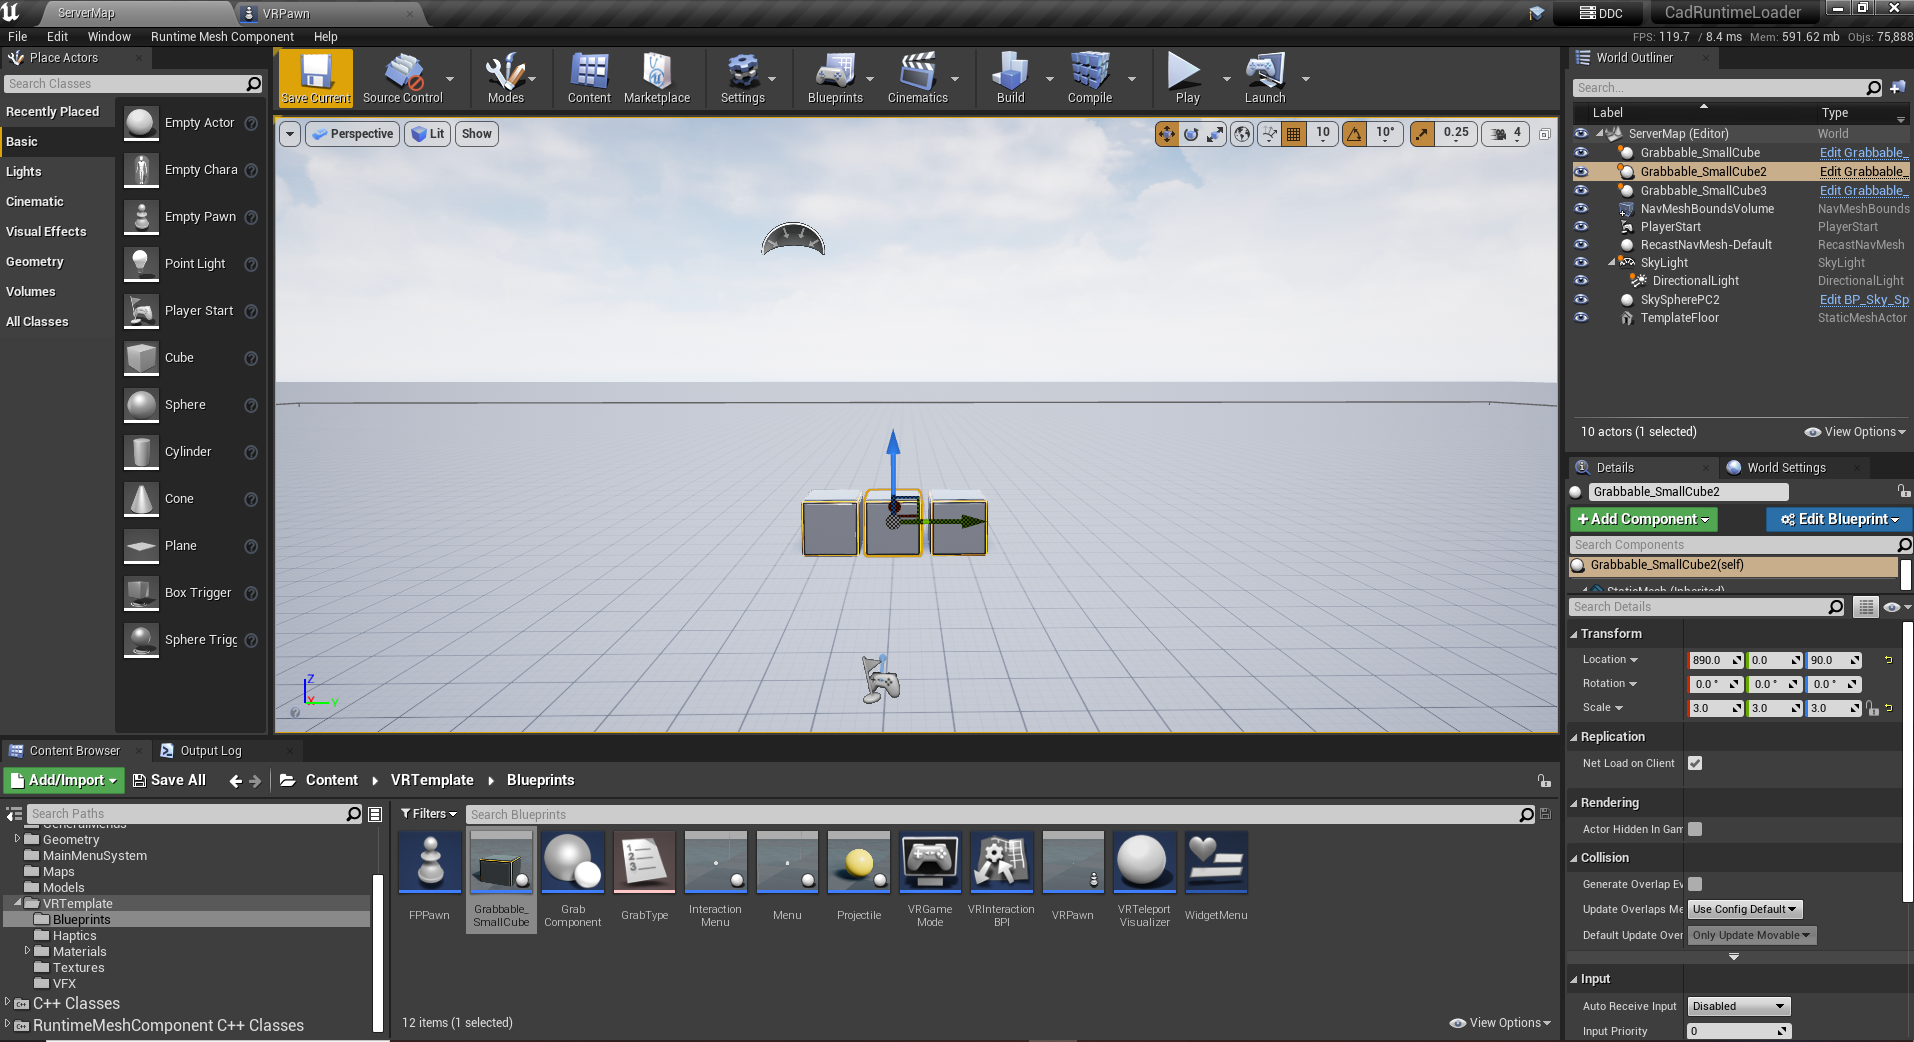
\includegraphics[width=0.9\textwidth]{fig/UnrealEngineLevelEditor.png}
	\caption[Unreal Engine Level Editor]{Example of what the Level Editor looks like for a project \protect}
	\label{fig:LevelEditor}
\end{figure}

\subsubsection{Actors and Components}

In Unreal Engine all of the objects that can be placed inside of a level are called Actors\cite{bib:UEActors}. This includes everything from meshes to particle systems to even the players starting location. This is partially due to Unreal Engines object-oriented nature so having all objects inherit from one base class, in this case Actor is beneficial. Actors can be created and destroyed through code and support 3D transformations like translation, scaling and rotation.\\

In order to add functionality to an Actor, so called Components are used\cite{bib:UEComponents}. Components can offer varying functionalities such as creating sounds, light or movement and once they are added to an Actor, the Actor can access these features and use them for its own purposes. It is important to note that a Component cannot exist on its own and an instance of a Component has to be attached to an instance of an Actor. It doesn't have to be directly attached though, as a Component itself can also have several subcomponents. So, the Components are what actually makes an Actor what it is supposed to be. Let's take a house as an example. All of the walls, floors, lights and other parts would be the Components, while the house as a whole is the Actor.\\

When an Actor is placed inside a level it gets a world transformation which describes the Actors location, scale and rotation in comparison to the world origin. A Component along with that also gets a relative transformation, which are again the same values as the world transformation but this time relative to the origin of its parent object. The world transformation of a Component can be calculated by adding the relative transformation to the parent's world transformation. This is very important to keep in mind when Components are moved around in a scene. 

\subsubsection{Pawns and Controllers}
Amongst all of the Actor subclasses, there are two which need to be especially highlighted. These are Pawns and Controllers and they form the basis of user-interaction in Unreal Engine.\\
The Pawn class is the base class for all Actors which can be controlled by a user or through \acs{AI}\cite{bib:UEPawn}. A Pawn determines what a user looks like visually and how they interact with their surroundings either through collision or other physical means. Generally, for Pawns that will be controlled by users, a further subclass called Character is used\cite{bib:UECharacter}. A Character has the additions of a Character Movement, Capsule and Skeletal Mesh Component. The Character Movement Component enables various means of moving like walking, flying, swimming for a character in a scene. It assumes that collision class is vertically-oriented capsule, described in the Capsule Component, and uses this for movement collision. The Skeletal Mesh simply allows for the use of more complex animations which require some sort of skeleton. What this looks like inside the editor can be seen in Figure \ref{fig:UnrealCharacter}. This is the basic template Unreal provides for a third-person character. Aside from the already mentioned Components, it also has an Arrow Component, which shows what direction is forwards for the character, and a Camera Component that represents where the view of a user will be during gameplay.\\

\begin{figure}[htpb]
	\centering
	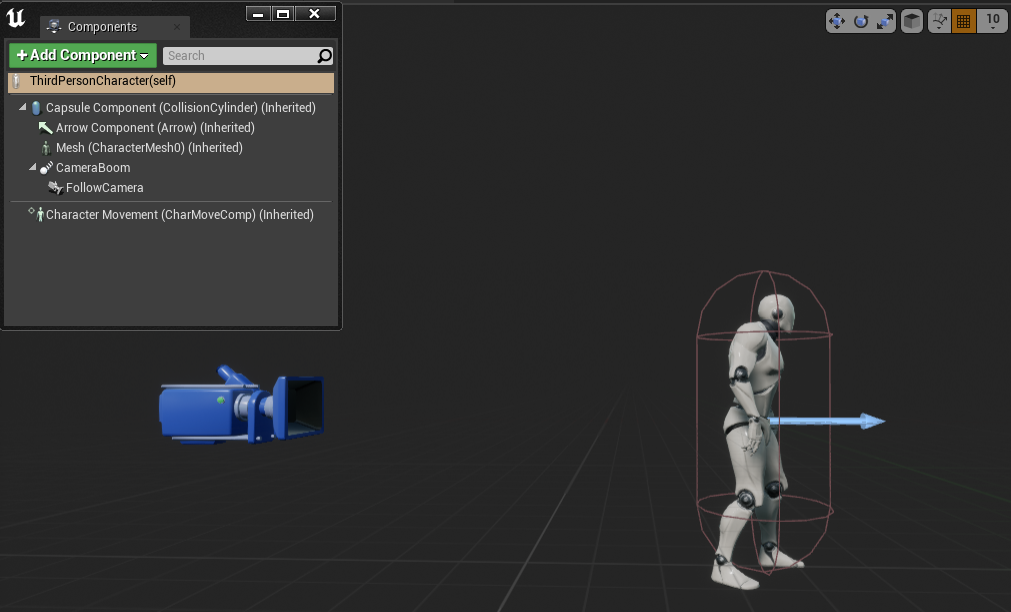
\includegraphics[width=0.9\textwidth]{fig/UnrealCharacter.png}
	\caption[Template for third person character]{Template for a third-person character\protect}
	\label{fig:UnrealCharacter}
\end{figure}

While some functionalities can already be implemented inside of a Pawn, this alone is not enough to get user inputs. For that an additional Actor called a Controller is necessary, specifically a Player Controller. A Player Controller is a non-physical Actor that functions as an interface between a human user and a Pawn\cite{bib:UEControllers}. Generally, there is a one-to-one relationship between a Player Controller and a Pawn. There are cases where this doesn't have to be the case but for the purposes of this project, that is not of interest. This relationship doesn't mean that a Controller can only ever possess one Pawn, just that it can only do one Pawn at a time. The process of gaining control over a Pawn is called `possessing' and losing control is called `unpossessing'. This, alongside slight differences between classes, is why it is important to properly choose whether certain functionalities should be implemented in the Pawn or the Controller.

\section{C++ and Blueprints}

Now that the most important design elements have been explained, the next step is to explain how writing code in Unreal Engine works. When it comes to this regard, Unreal has a rather unique combination of programming tools with C++ and its own Blueprint Visual Scripting system. As already mentioned, Unreal is written in C++ so it makes sense that it would also be used for its programming. What is important to note is the fact that it is not pure C++. Rather, Unreal Engine has developed its own extensive C++ \acs{API}, also known as Unreal C++, tailored for game development built upon normal C++\cite{bib:UECPlus}. This \acs{API} provides libraries for common game development features as well as many built-in classes, functions and utilities. The idea behind this is to have a fully functioning framework that makes the developing process simpler and faster than it would've been using standard C++. An excellent example of this is the fact the Unreal C++ supports multiplayer and network replication on a core engine level.\\

The other way to program in Unreal Engine is the Blueprint Visual Scripting system, more commonly referred to as Blueprints\cite{bib:UEBlueprints}. This system is a relatively new addition to Unreal as it was first released with the launch of Unreal Engine 4. It was meant to be a replacement for the previous Kismet scripting system which was complicated and outdated\cite{bib:UEBlueChanges}. Blueprints, like many visual scripting languages, use an object-oriented approach for developing. It is a powerful and flexible tool which is meant to allow designers to create impressive gameplay elements without needing to know how to program\cite{bib:UEBlueprints}. As such it has access to almost all the same frameworks and APIs C++ has. This means that whole games and projects could be made only using blueprints. Likewise, the same could also be done with only C++ but such approaches are generally not advised. There is a reason after all why Unreal specifically has both tools and they each have their purposes in development. C++ is advantageous when designing base systems for a project and for writing performance critical features. On the other hand, Blueprints shine when they are used to design the behaviour and incorporate it into the rest of the program. Another great benefit of Blueprints is that, due to their simplicity, they allow for rapid prototyping and then these prototypes can easily be translated into C++ if the increased performance is necessary.\\
Due to this unique mix of tools, a typical workflow for creating features would look as follows. First a C++ programmer would create a new class, add the required features and properties and then ensure that they can properly be accessed in the Blueprints. An example of a header for such a class is shown in Figure \ref{fig:ClassExample}.
\begin{figure}[htpb]
	\centering
	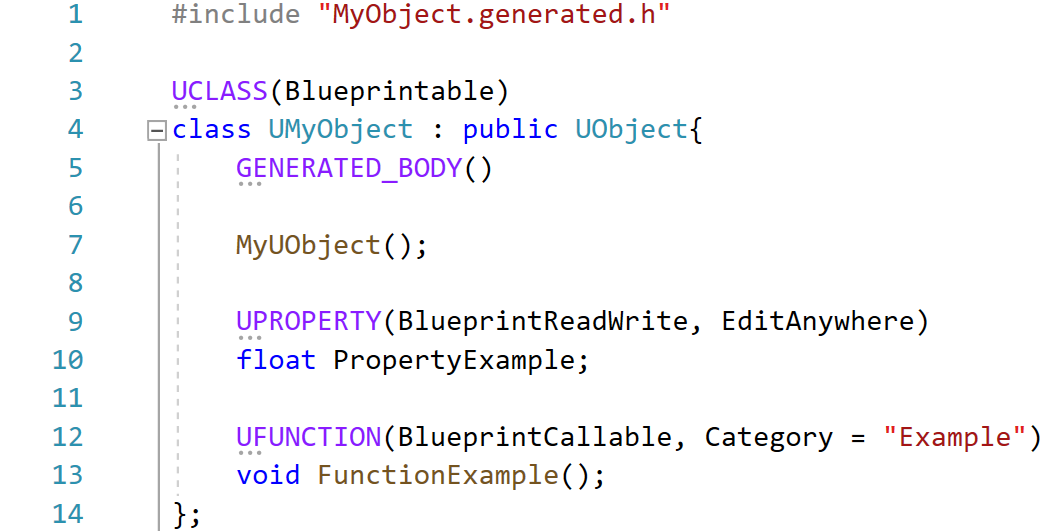
\includegraphics[width=0.8\textwidth,height=160pt]{fig/ClassExample3.png}
	\caption[Example Unreal C++ Class Header]{Example Unreal C++ Class Header\protect}
	\label{fig:ClassExample}
\end{figure}
As can be seen, the code does resemble normal C++ header code with a few special lines. Most important are the macros that can be found in the 3rd, 9th and 12th line of code. These special lines of code are used to describe the class, property or function in the line below them. This description is used by the Unreal Editor to determine if and how these objects should be presented in Blueprints. As an example, the property is set to "BlueprintReadWrite" so that it can be read and modified in Blueprints. There are many specifiers that can be used depending on what the desired outcome is and it is important that these are used properly to mitigate possible problems.\\
 
Once that part of the development is done, the new class can be used in the engine. The class itself, seeing as it is C++ code, can't be directly worked within the Blueprint editor. Instead, a new Blueprint class needs to be made that inherits from the C++ class and then that new class can be opened in the editor.\\
As previously mentioned, Blueprints are a visual scripting system, which means that the code isn't represented through text but rather with nodes which are connected among each other. An example as to how this looks like in the Blueprint editor is shown in Figure \ref{fig:BlueprintExample}.

\begin{figure}[htpb]
	\centering
	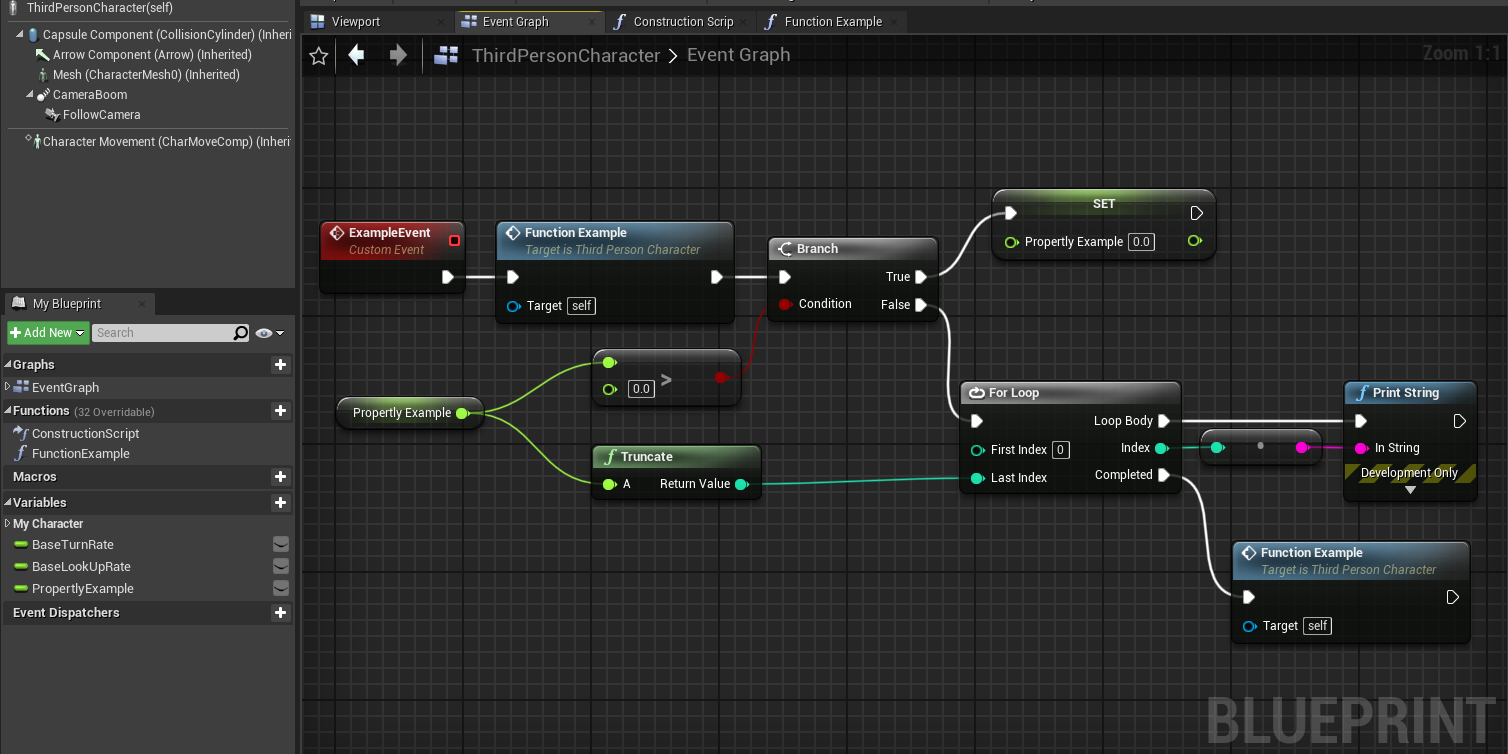
\includegraphics[width=0.9\textwidth]{fig/BlueprintExample.png}
	\caption[Example Blueprint Code]{Example of Blueprint Code in the Blueprint Editor\protect}
	\label{fig:BlueprintExample}
\end{figure}

At the top left side of the screen the Components of the current Actor can be seen. Underneath that is an overview of all the functions, graphs and variables contained in the blueprint. In the centre of the editor is the event graph of the class, this is where all the various events that can happen to it are handled. In the example shown it needs to be noted that the view is heavily zoomed into a single event in order to better see the individual nodes. Typically, there will be many events all across the graph and also sub-graphs to keep the code readable.\\
The execution flow of the code is represented by the white line connecting the nodes. The nodes themselves have varying functions and are colour coded accordingly for better understanding. Red nodes represent the starting point of an event. This can be triggered by many actions including collision, player inputs or other events. Blue nodes are either functions or event calls and green nodes are usually used for retrieving values. Lastly grey nodes represent macros or flow control nodes. This is where the typical programming tools such as \textit{if} conditions, \textit{for} and \textit{while} loops can be found.
Depending on if they are needed, \textit{input} and \textit{output} pins can respectively be found on the left and right side of a node. These are connected using lines that automatically match the colour of the value, which are also colour coded, and can only be connected to other pins of the correct type.\\
All in all, these properties and features make using Blueprints quite simple and almost play-like, which makes them accessible to a wider audience, while staying quite powerful.

\section{Networking}

Everything that was discussed so far mostly relates to what happens in a single instance of our program. Nonetheless networking is a big part of the Unreal Engine and is required to understand the steps that are needed in order to create a multi-user project.\\

When the program runs in a standalone mode, all of the objects that make it up exist on the local machine which is running the program and only on that machine. For a network multi-user program, Unreal Engine uses a so-called client-server model\cite{bib:NetworkComp}. One computer acts as a server and hosts a session that can be joined by other user as clients. The server is what connects all of the different users and enables their communication with each other. The instance running on the server is the true, authoritative world instance. In other words this is where the multiplayer is actually happening. The clients only have copies of this world. The server tells the clients what Actors exist, how they should behave and what values their variables should have. The clients then use this information to approximate what is happening on the server in their own copy of the world. The clients only really control the Pawn and Player Controller that they are assigned to. One thing to note is that while a copy of a Pawn exists in every instance of the program, the Player Controller only exists for the owning player and server. This means that a local Player Controller is completely unaware of the existence of other Player Controllers.\\

In total there are three network modes in which an Unreal project can run in: standalone, client and server\cite{bib:NetworkComp}. For the server mode there is a further classification into listen and dedicated servers. A listen server represents a user hosting a session through their local machine. This means that they function both as a server and a client simultaneously. The benefit of this is its relative simplicity, especially with Unreal's already existing tools and support for many popular online subsystems such as Google, Amazon and Steam\cite{bib:UEOnlSuS}. A big downside of this approach is the extra load that is put on the server machine, as it also has to handle user-relevant features like graphics. Also, the user that hosts the server can get a slight advantage from the non-existent latency, although this is only relevant in specific circumstances.\\
A dedicated server on the other hand runs ``headlessly", which means it does not have to render any visuals and isn't controlled by anyone locally. This means that most of the resources available to the machine can be used for hosting and moderating the program. Unfortunately, this requires a separate computer with its own network connection, not to mention a lot of complex work to be properly configured.\\

\begin{figure}[htpb]
	\centering
	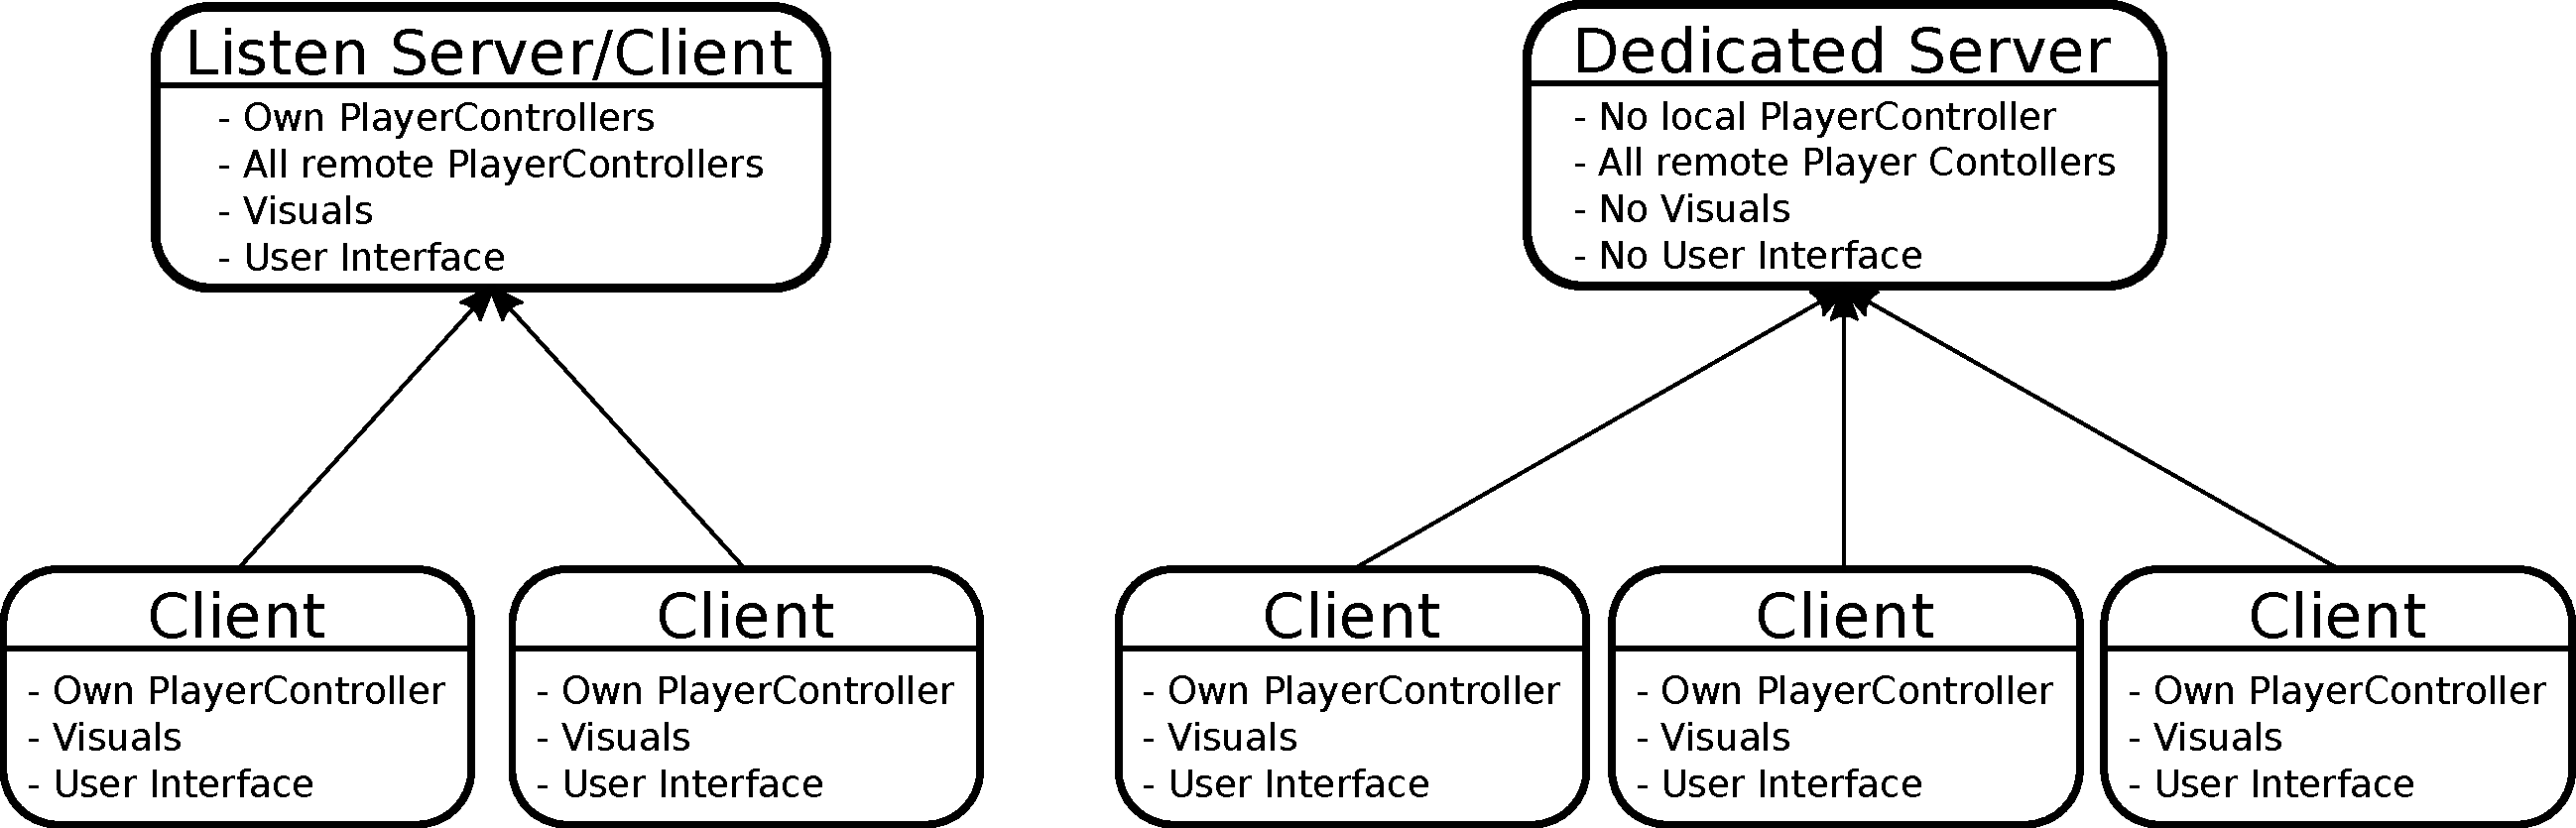
\includegraphics[width=0.8\textwidth]{fig/ListenvsDedicated.pdf}
	\caption[Difference between Listen and Dedicated Server]{Example to demonstrate differences between a Listen and Dedicated server\protect}
	\label{fig:ListenvDedicated}
\end{figure}

The actual information sharing and interaction between users through a server is done through replication and remote procedure calls\cite{bib:NetworkComp}. In order to use replication for a variable, its boolean specifier ``Replicated" ~needs to be set to true. Now when the variable's value is changed on an authoritative Actor, usually on the server, the change is automatically sent to the connected remote copies of the Actor. If a variable is changed locally in a client's instance, this will not be replicated to the server or other clients. This doesn't mean that every variable needs to be replicated, as that could cause problems in network traffic. Rather it is important to use replication carefully and replicate only variables that require it.\\
\acp{RPC} are functions which are called from a machine but executed remotely on another machine. They are also known as replicated functions\cite{bib:NetworkComp}. In order for a function to become an RPC, the keywords server, client or multicast need to be added to its definition. The server and client keywords simply mean that the function should be executed specifically on the server or on the client. Multicast means that a function will be called on every instance of an object. Another peculiarity of RPCs is that they have no return value. In order to achieve that another RPC is needed which returns the output from the remote to the local machine.\\
All of this is only a small section of all the features that Unreal Engine is capable of but for the purposes of this project, this should suffice as an introduction to the engine and make understanding the rest of the work easier.




% replications, rpcs,
\newpage
\newpage\thispagestyle{empty}\hspace{1em}\newpage
\chapter{Dynamic 3D Object Insertion}\label{chp:ObjectLoading}

In order to realize the insertion of a 3D object from a CAD file, a plug-in with this functionality was developed simply called CADRuntimeImporter(CRI). Alongside it a standalone Unreal prototype project, named CADRuntimePresenter(CRP), was made that incorporates CRI in order to demonstrate how it can be used for a multi-user desktop and VR environment. The whole mechanism can be split into three major sections: opening and parsing the files, generating the objects and lastly user interaction with said objects. How all of that was implemented and what sort of advantages and disadvantages these approaches have, will be discussed in this chapter.
%%%%%%%%%%%%%%%%%%%%%%%%%%%%%%%%%%%%%%%%%%%%%%%%%%%%%%%%%%%%%%%%%%%%%%%%%%%%%%%%%%%%%%%%%%%%%%%%%%%%%%
\section{Loading and Parsing CAD Files}
\subsection{File Loading and Sharing}
The first step in creating an object in runtime is naturally opening the desired file and getting the required data from it in runtime. As Unreal Engine is written in C++, it is not surprising that opening up a file isn't too much of an issue. What makes this simpler is the fact that Unreal also offers this in their FileHelper class with the functions LoadFileToString() and LoadFileToArray(). The first function can load a text file into a string, while the other loads binary files into an array of bytes. This is only directly available in C++ and therefore had to be exposed to Blueprints. As this functionality is more of a utility, it isn't the best idea to attach it to a specific object. Luckily for such purposes Unreal offers Blueprint Function Libraries. This is just a special type of Unreal C++ class in which only static functions can be defined. These functions then become available to be used in any Blueprint without needing any instanced objects.\\

Something that is slightly more complicated is actually choosing the file. Here Unreal does technically offer the ability to open a file dialog but this is a strictly developer only module and can't be used in finished products. Even neglecting that, it wouldn't work in VR so a separate solution would have been needed anyway. Due to this a file picker in CRPs UI had to be written. The end result of that can be seen in Figure \ref{fig:FilePicker}. The design is rather simple but offers all the necessary functionality, especially that it is compatible with VR and only displays supported file formats.\\

\begin{figure}[htpb]
	\centering
	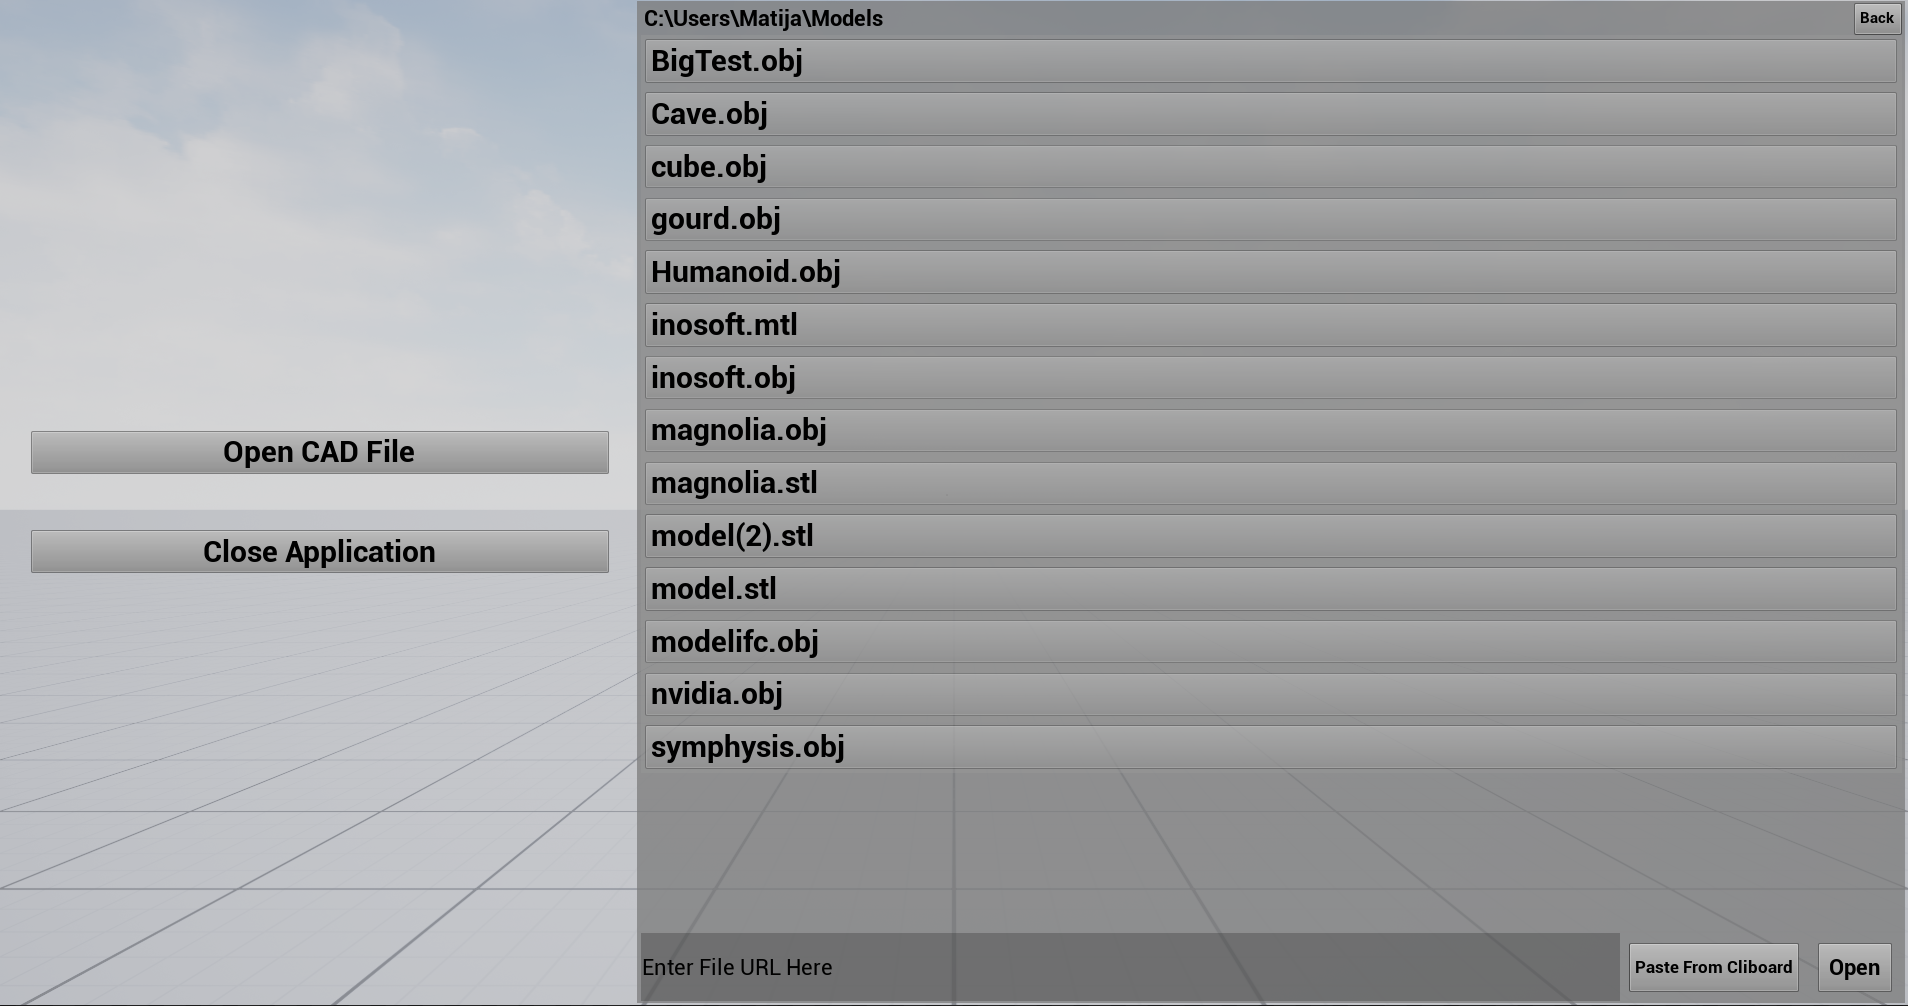
\includegraphics[width=0.9\textwidth]{fig/FilePicker2.png}
	\caption[CAD Runtime Presenter File Picker]{File Picker for CRP\protect}
	\label{fig:FilePicker}
\end{figure}

For a single user this would be enough, they could choose a file and then it could be parsed for object generation. Complications arise once there are multiple users involved. If a user were to open a file in such a scenario, the object would appear only in the world of that user and not for other users or even on the server. This could cause many issues since the clients world would not match servers, which is the authoritative instance. The problem lies in the fact that the new object needs to be created on every client and on the server. In order for that to happen every machine needs access to the required data, not just the client who has the file available on their machine.\\

One way of sharing this data is saving it in a replicated variable and having it handled by the automatic replication system. This does actually work but it has one fatal flaw which makes using it not viable. That is the size limit of replicated variables. The size limit for arrays is 64 kilobytes and for strings it seems to about the same. For smaller files this would be a perfect solution but unfortunately CAD files tend to be too big for it.\\
So instead this problem was solved by having the file be uploaded to a server and then be downloaded by the rest of the clients and server. For such purposes Unreal offers the HTTPModule interface, which uses the popular and powerful libcurl library, to create HTTP requests. A file could then be uploaded using a POST request and downloaded using a GET request. For this a simple file server which can handle such requests was written in python. The only problem is that the clients and server need to know where and what file was uploaded in order to make the correct request. This is where replication comes in handy. The client that uploads the file can tell the server where it was uploaded through a replicated string, which is most likely going to be within the size limit, and then the server can propagate that information to the rest of the clients which then make the GET requests.\\
Seeing as for most users only the link to the file matters, this means that the client that wants to open a file doesn't even need to have it locally on their machine. Instead they can simply input a link to a service like Dropbox or Google Drive and have everyone download those files. The UI for that is also part of the file picker and can be seen at the bottom of Figure \ref{fig:FilePicker}.\\
There are technically other libraries and plug-ins that could be used to enable file sharing with more complicated protocols but that wasn't necessary for this prototype project. The HTTPModule is simple to use while offering all the needed functionalities and avoids having to rely too much on third-party libraries.


%%%%%%%%%%%%%%%%%%%%%%%%%%%%%%%%%%%%%%%%%%%%%%%%%%%%%%%%%%%%%%%%%%%%%%%%%%%%%%%%%%%%%%%%%%%%%%%%%%%%%%
\subsection{Parsing Wavefront OBJ and STL}

Once every instance of the program has the desired file, the next step can begin which is parsing the data. What data is available and how it is stored can vary heavily from format to format. Generally they will all have the vertices that define the mesh but outside of that colour, material or anything else isn't guaranteed. This is the case because CAD formats tend to be highly specific for their uses cases, as well as proprietary for the CAD software they were developed for. This makes supporting many CAD formats quite difficult, especially those that aren't well documented or don't even have publicly available documentation. Considering the scope of this project, spending too much time writing parsers for as many formats as possible was not feasible.\\
Instead the decision was made to use well known and widely supported formats, like OBJ and STL. One of the biggest benefits of this approach is the already existing support that these formats have. Many CAD softwares support exporting to one of these and even if they don't, there are probably tools with which the files can be converted. This saved a lot of time in the development, as only a few parsers had to be written and for those that had to be implemented, the process was fairly simple due to all the existing resources on the formats.

\subsubsection{Wavefront OBJ}

Wavefront OBJ, or simply OBJ, is a geometry definition file format developed by Wavefront Technologies for their Advanced Visualizer animation packages. It is a neutral, open source format which has been widely adopted and has good import and export support from almost all CAD software.\\
Another reason why OBJ was chosen is the fact that is can be directly read through any text editor. This helped out a lot in early stages of development where the primary goal was to prove that the concept worked. Being able to see and read the data made it simpler to write a parser in the first place, as well as comprehending what was going on with the data at later stages.\\ 
The format represents 3D geometry in the form of vertex positions, vertex normals, texture coordinates, polygonal faces and groups of faces. These geometries can also use materials indirectly through referencing materials defined in a separate MTL file. Every entry in an OBJ file is represented through a single line, starting with an identifying tag followed by the value of the entry. What these entries can look like is represented in Table \ref{tab:ObjTypes}.

\begin{table}[htbp]
	\centering 
	\scalebox{0.889}{
		\begin{tabular}{lll}
			\toprule \textbf{Tag} & \textbf{Example Value} & \textbf{Definition} \\
			\bottomrule
			v & 0.2 0.3 0.5 & 3D Vector representing 3D Vertex \\
			vn & 1.0 0.5 0.0 & 3D Vector representing 3D Normal \\
			vt & 0.5 0.25 & 2D Vector representing Texture Coordinate\\
			f & 1/1/2  2/2/5  3/3/5 & Polygonal Face made from Vertices, Normals and Textures\\
			usemtl & Stone & Defines what Material should be used for following faces\\
			g & Door & Defines a polygon group\\
			\bottomrule
	\end{tabular}}
	\caption[ObjTypes]{Relevant types in OBJ format}
	\label{tab:ObjTypes}
\end{table}

In order to parse their values, most of the entries can be regarded one-by-one. Vertices, normals and texture coordinates are vectors and can be saved in separate vector arrays in the order in which they appear. How these and the rest of the values are used will be explained later, for now it's only important how they are saved.\\
Faces, materials and group are more complicated as they define how the rest of the data is put together to make the object. A face represents a polygon defined through lists of vertex, texture and normal indices in the format "vertexIndex/textureIndex/normalIndex", as can be seen in Table \ref{tab:ObjTypes}. It is important to note that these are the indices of the values and not the values themselves. Also the indices for vertices, texture coordinates and normals are separate and based on when the entry was defined in the file starting with one. So both a vector and normal can have their respective index be 1. The polygons themselves tend to be triangles but can also have more sides. This isn't ideal as later for generating the mesh, only triangles are supported but there is a simple way to solve this. The vertices are listed in a counter clockwise order so that any polygon can be represented through a triangle fan, as is shown in Figure \ref{fig:TriangleFan}. So faces that define polygons with more than 3 edges are replaced through multiple triangular faces.

\begin{figure}[htpb]
	\centering
	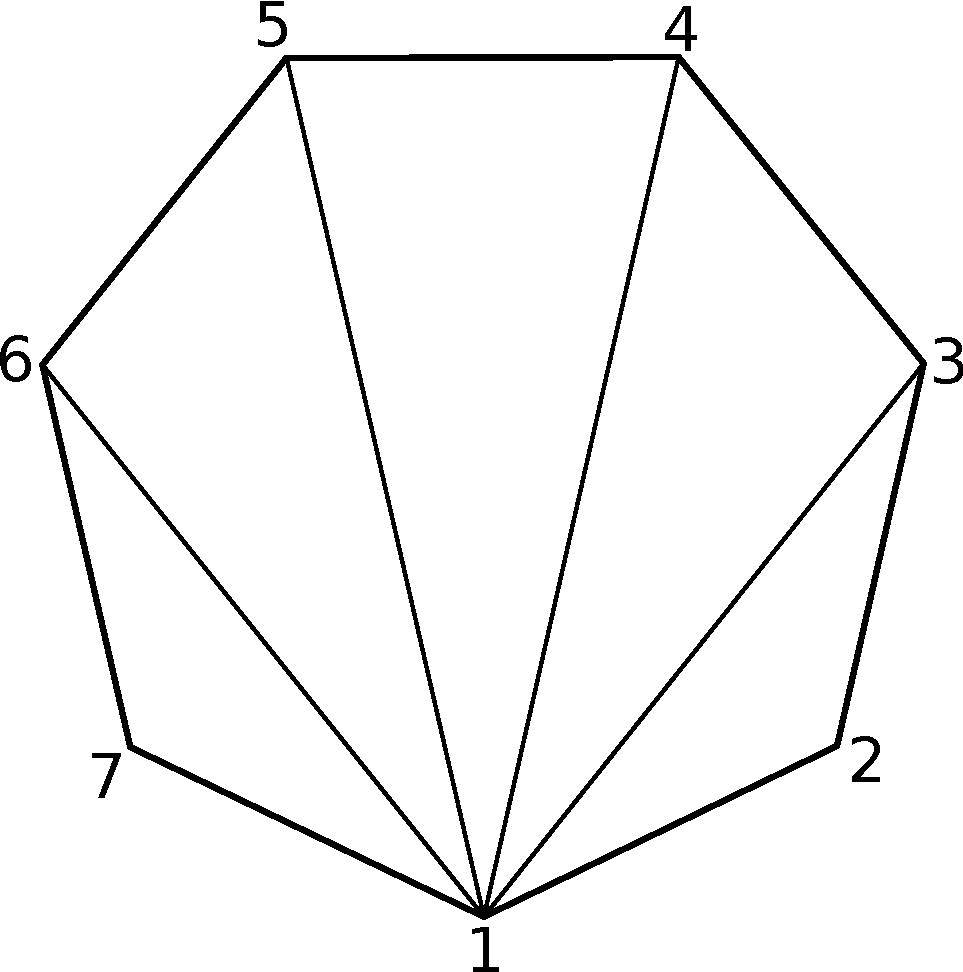
\includegraphics[width=0.3\textwidth]{fig/TriangleFan.pdf}
	\caption[OBJ Polygon to Triangle Fan]{Polygon represented through a Triangle Fan\protect}
	\label{fig:TriangleFan}
\end{figure}

A group determines what faces are combined in order to make a component of the larger object. The "usemtl" tags tells what material should be used on the faces and that material is used until the next tag appears. The actual materials are defined in an MTL file, which works similarly to an OBJ, just with different tags and values. Some of the more important entries can be seen in Table \ref{tab:MTLTypes}. This MTL file of course also needs to be shared to every client. The values themselves are saved in a Map where the keys are the material names and the values are arrays of the values.

\begin{table}[htbp]
	\centering 
	\scalebox{0.889}{
		\begin{tabular}{lll}
			\toprule \textbf{Tag} & \textbf{Example Value} & \textbf{Definition} \\
			\bottomrule
			newmtl & Stone & Defines the name of a new Material\\
			Ka & 1.0 1.0 1.0 & Ambient colour\\
			Kd & 0.0 0.0 0.0 &  Diffuse Colour\\
			Ns & 1.0 & Specular Exponent\\
			d & 0.5 & Transparency\\
			
			\bottomrule
	\end{tabular}}
	\caption[MTL Types]{Relevant types in MTL format}
	\label{tab:MTLTypes}
\end{table}

As the information of these values heavily relies on each other, they needed to be combined and saved in an array where every array entry represents one component of the whole object. The entry consists of the face values and marks where materials need to be switched.\\
The only major problem with OBJ is the fact that the coordinates don't have units, meaning they can't be scaled to properly represent the designed size. Instead everything is scaled with same factor so that at least the scales between objects made in the same scene stay the same. Also the created objects can later be scaled by users to better resemble the desired size.

\subsubsection{STL}
STL is a file format native to the CAD software created by 3D Systems in 1987\cite{}. The format has gained a lot of support in many different software packages, especially for 3D printing software where it is one of the default formats. STL files only describe the surface geometry of a three-dimensional object with out any additional information about colours, materials or groups. The geometry is described in raw, unstructured triangles defined by a normal and three vertices. The way a triangle is defined in the file is shown in Figure \ref{fig:STLFormat}. 
\begin{figure}[htpb]
	\centering
	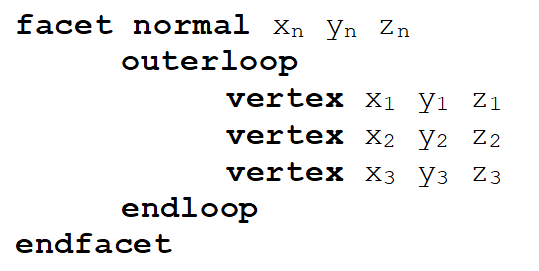
\includegraphics[width=0.35\textwidth]{fig/STLFormat.png}
	\caption[STL Triangle facet]{A triangle facet represented in STL\protect}
	\label{fig:STLFormat}
\end{figure}

While the structure suggests that multiple possibilities are possible for loops, the facets can only be triangles. In order to represent a full model the triangles are simply listed one after the other. In order to parse it, the vertices and normals are saved in arrays and faces are generated to point what vertices make up the triangles. This is important for generating the mesh later. While it is a simpler format compared to OBJ, it is excellent when only the shape is relevant. It does unfortunately suffer from the same scaling problems as OBJ and that is handled in the same way as well.\\
Overall with these two formats the majority of the most common and well-known CAD formats are covered. Ideally more formats would be covered and specific parsers for every format would be written to get the most accurate results but for the limitations of this project, this is a very practical solution.

%%%%%%%%%%%%%%%%%%%%%%%%%%%%%%%%%%%%%%%%%%%%%%%%%%%%%%%%%%%%%%%%%%%%%%%%%%%%%%%%%%%%%%%%%%%%%%%%%%%%%%%%%%%%%%
\section{Runtime Mesh Generation}

After the files have been parsed and the needed data was extracted, the actual process of creating a new 3D object starts. For that, a way to tell Unreal to generate a mesh is required and Unreal does in fact support such a feature in the form of so called Procedural Mesh Components(PMC). These components can be created in runtime by giving them the required mesh data and letting them generate themselves. In the first phases of this project it was explored as to how viable using these components were, seeing as they initially seemed to be exactly what was needed. Getting it to function took a bit of work, mostly due to Unreal Engines generally bad documentation, but the first results with small objects were quite promising. Unfortunately the problems started to arise with larger objects where the performance would drop significantly or the Unreal editor would simply crash. The reason for this lies within the procedural mesh components themselves. As the name implies, these components are supposed to be generated by some form of procedure which generally won't create nearly as many vertices as a large CAD file can. On top of that the underlying architecture for a real procedural system for expensive geometrical operations would be quite different to that of a runtime gameplay framework \cite{}. PMC is also a relatively late addition to Unreal Engine, first appearing in version 4.8 in 2015. So even though it is designed for a quite similar purpose, it is different enough that it couldn't be used.\\

Due to this a different method of getting Unreal to generate meshes had to be found and during this time a the most important question for this project came up. Doesn't Unreal technically already support runtime mesh generation? Let's say, as an example, there was an Actor that had some sort of static mesh attached to it. Unreal could spawn in this new Actor without a problem. So shouldn't it be able to create such an Actor from data parsed from a file?\\
A definitive answer for that question couldn't be found but through some research a few speculations can be made. The biggest reason for this probably stems from the main purpose of Unreal Engine. Unreal has always and will probably always be a video game engine. As such it is designed and optimized for use cases that happen in video games. In a game, every asset and model is carefully crafted and placed in a level. These objects are already known to the game and are packaged within it in an optimized state. The game knows exactly what to do with these and where to load them. That is a part of the core functionality of Unreal. But it isn't exposed directly to a developer because adding externals models to a game isn't generally required. Why should a game depend on the user having some specific type of file to load? Those need to be within the game itself. Not to mention the problems and security issues an external file could cause.\\
Another factor that comes into play are the hardware limitations that existed throughout most of Unreal's lifespan. Computers and gaming consoles weren't always as powerful as they are now, especially consoles tend to be very underpowered machines. As such a lot of work went into optimizing games so that they would run smoothly on their target platforms. Even nowadays with modern systems that are way faster, optimizing is a big part of game development. Especially important for that is managing what is loaded in and when as the systems can have limited memory. Some games will use a loading screen to hide the loading, other games might use a gameplay sequence that slows down the player so the game has time to load in the next assets. There are even games that would restart the console they were running on without letting the player know when the memory was full\cite{}. How these assets were stored also played a big role. Some games would use the same asset but with different colours to save space or some games saved the same asset multiple times so it could be accessed from storage quicker\cite{}. CAD files on the other hand tend to be rather big and just creating the files is already a very demanding job which requires good hardware. Due to all of this, the idea of just creating a new external model using Unreal's functionality isn't of value to game development and isn't directly exposed.\\
However Unreal isn't just a game engine any more. As already mentioned it has gained popularity in various fields and those have very different demands compared to games. This has led to many new additions to Unreal, most importantly Datasmith. Datasmith is a set of tools and plug-ins developed by Epic Games with the goal of streamlining the process of importing CAD files into the engine during development. It is a relatively new addition to Unreal as it was first released around 2016. CAD objects are very different to objects used in game development, they focus on creating geometry for manufacturing and production while game objects are more focused on looking a certain way and being optimized. Due to this, it is clear that this addition isn't meant for game development. But it wasn't until August of 2021 with the release of Unreal Engine version 4.27 and with it the release of the Datasmith Runtime plug-in that it gained the ability to import meshes in runtime. This plug-in, as it is still very new, is in beta and still being worked on. Most importantly it shows that with access to the mesh generation functionality of Unreal it is possible to create meshes from external data in runtime.\\ 

But the demand for such a functionality has existed for a lot longer and Unreal's existing solution with PMC wasn't good enough, which led to the development of Runtime Mesh Component (RMC). RMC is a third-party plug-in developed that exposes the mesh generation capabilities of Unreal in a much more efficient and feature-rich way compared to PMC. It promises 50-90 \% lower memory usage and 30-100 \% lower render thread CPU time \cite{} compared to PMC. These claims were checked and the results do match the expected improvements. It is also completely free and has been used in many projects even in larger companies \cite{}. This is why it was finally decided to use RMC for the purposes of this project. While ideally this project wouldn't need to rely on an unofficial plug-in, trying to recreate what is available with RMC, which has been around for more than 6 years and had more than 40 people contribute it, is not a feasible endeavour. Instead, for the limitations of this project, it is much wiser to use this tool and apply its  capabilities for the purposes of generating CAD models.

\subsubsection{Generating a CAD Model}

% setiing up the class
%generating componenet individually through function sections
%attaching it and making it part of the actor
%setting it's relative position and setting the components 
%sections differ based on material as only one material per section is allowed
% creating the materials
Before a model can be generated, there needs to be an Actor to which the components can be attached to. Technically this could be any Actor, even the Player Character, but it makes more sense to create a specific Actor for these purposes. In the plug-in such an Actor is defined in the CRIObject Blueprint class. Actors of this class are also going to be where the values from the parsed files will be stored, as well as the Actors that call the function to generate the new components on themselves.\\
In order to spawn in a new Actor of this class, the Unreal SpawnActor function can be used. This function just needs to know what class should be spawned and where. The first parameter is easy but the second one has a few more options. Depending on what is needed all these Actors could be spawned in the same place or a user could enter the coordinates. For the purposes of CRP it was decided that the location of the new Actor is going to be where the user adding the object is looking. For this the users camera rotation is taken as a forward vector, multiplied by a distance and added to the players location. The distance is based on the size of the spawned object so that collision is avoided but it also isn't spawned to far from the user. Also this spawning process happens as soon as clients start downloading the CAD files so that once the files are parsed, there is a place to save the data. The Actors will be in the world but won't be visible or interactive as they don't have any components yet.\\
Once the data has been saved, flags in the Actor get set in order to notify it that generating can begin. This is done because there is no guarantee that the CAD and material file will be downloaded in any specific order and generating before all the needed data is there would cause problems. The material flag is also only used if the file uses it and the user specified that it should be created with materials.\\
The whole model isn't generated all at once because this could cause the program to stutter or freeze for the duration of the process for larger files. This happens due to this running on the same thread as the main thread, which means that nothing is rendered until this is finished. Instead each component gets generated separately from the rest in the order that they are defined in the file. This is realized through the tick event that Actors can possess. A tick event is simply an event that gets called every frame or in some other interval. As the components themselves are comparatively small, generating one doesn't cause a significant performance hit that could freeze the main thread. So basically by doing this, the performance cost of generating the model gets spread across every component and becomes practically negligible. Another benefit of this is the fact that the components themself start appearing one after the other in the world, creating an interesting-looking animation. Ideally multithreading would be used for even better results but Unreal is rather specific about that due to its built-in garbage collection\cite{}.\\
With every tick the GenerateMeshComponent function is called and a counter is kept as to know what components have already been dealt with. The function is implemented in C++ as the performance is necessary but in order to call it from Blueprints it was implemented in a Blueprint Function library, just like the file reading function. It could also have been implemented as a native function of the CRIObject class but, as this is supposed to function as a plug-in, it didn't make sense to limit it to one specific class. This way the functionality can be used in more ways depending on what the user needs. One such way is implemented in CRP and will be demonstrated later.\\
How the function works can be seen in Algorithm \ref{algo:MeshGeneration} which shows the process in a simplified pseudocode.

\begin{algorithm}[htpb]
	\texttt{Input} $Actor, ComponentIndex, Vertices, TextCoords, Normals, \linebreak \null \quad\quad \quad ComponentData, Materials, UseCollision;$\\
	$RMC = new \: CustomRuntimeMeshComponent()$\\
	$RMC.ID = ComponentIndex$\\
	$RMC.AttachTo(Actor)$\\
	$RMC.UseCollision = UseCollision$\\
	$Center = FindBoundingBoxMiddle()$\\
	$RMC.SetRelativeLocation(Center)$\\
	$Vertices.Translate(-Center)$\\
	$RMC.CenterVertex = Center$\\
	$Secitons = GetComponentSections(ComponentData)$\\
	$SectionMaterials = GetSectionMaterials(Materials)$\\
	\texttt{for} $i := 0$ \texttt{to} $Sections.Length$ ~\texttt{do}\\
	\hspace{5mm} $Faces = GetFacesForSection(Sections[i])$\\
	\hspace{5mm} $Material = SetupSectionMaterial(ComponentMaterials[i])$\\
	\hspace{5mm} $RMC.CreateSection(i, Vertices, Faces, Normals, TexCoords, Material)\newline$\\
	
	\caption{Pseudocode for generating a Mesh Component}
	\label{algo:MeshGeneration}
\end{algorithm}

As can be seen the function takes quite a few inputs but all of those necessary. The first step is instancing a new Runtime Mesh Component object. In this case it is a slightly customized subclass of RMC that contains a few more variables that can be quite useful. One of those being the index of component, which is used when interacting with components. After that the component is attached to the Actor generating it as it cannot exist in a scene on its own. Based on user wishes the mesh can be created either with or without collision. Next the a bounding box is generated from the vertices of the component and the centre of that box is determined. This is done because when a component is added to an Actor, its relative location is (0,0,0) so it's in the centre of the Actor. The mesh on other hand will be placed where the vertices are. Once the whole mesh is generated it will look exactly the way it should but there will be problems with certain interaction. Let's take rotation as an example. Since the position of the component is technically in the centre of the object, rotating it will cause the mesh to rotate around the whole object instead of itself. In order to fix that, the component is placed where the centre of the mesh will be and the vertices are translated the same amount just in the opposite direction. These two translations cancel each other out so that the whole mesh ends up looking unchanged. Meanwhile the position of the component matches the centre of the mesh so that rotating and scaling work properly. Alternatively the component could be moved and translated in specific ways to simulate such a rotation but this is many times more complicated and unnecessary. The location of the centre is also saved in the custom class as it is required for some interactions that will be explained later.\\
Then the component is split into sections and the material values for the sections are extracted. An RMC can contain one or multiple meshes and these are regraded as sections. In this case the mesh is split according to the materials seeing as a section can only use one material. This way a component can have multiple meshes, instead of having to create a component for every material change. Lastly for every section, all the indices defining its faces are saved in one array and the appropriate material for it is setup. In Unreal a completely new material cannot be created at runtime. Instead an already existing material is needed as the parent for an instance of a dynamic material. Such a dynamic material can be create during gameplay and the values that define it can be altered as well. There is just a slight problem du to the plug-ins current limitations. The materials in Unreal are physically based rendering(PBR) materials, while the MTL uses Phong shaded materials. These two ways of rendering are vastly different and there isn't one true way of converting between them. That's why the diffuse colour, specular exponent and opacity are used to approximate the appropriate values for the PBR material. How well this works depends on what material is supposed to be represented. This is slightly unfortunate but what is more important is the fact that an appropriate material could technically be created. If a new format, that supports PBR, were to be added the whole mesh generating approach would still be the same just with the correct values. Also technically two parent material are needed, one for opaque and one for translucent materials because of the way Unreal handles opacity.\\
Finally the RMC takes all of the inputs that it needs and creates a section. This is then repeated for every section of every component until the whole mesh has finished generating. The model will appear in the world in the position where the Actor was spawned and the result of such a process can be seen in Figure \ref{fig:LoadedModel}.

\begin{figure}[htpb]
	\centering
	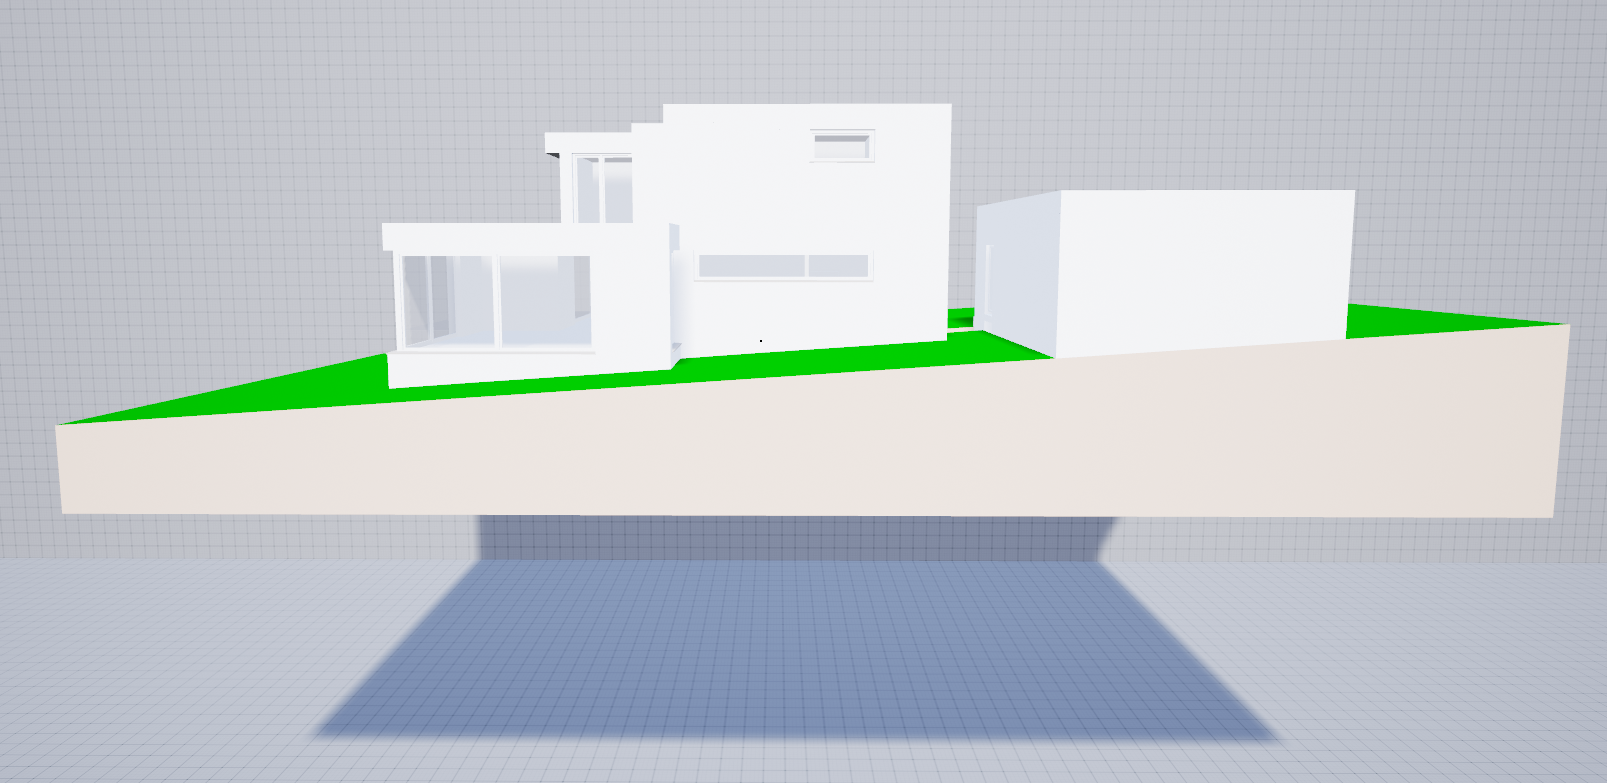
\includegraphics[width=0.675\textwidth]{fig/LoadedModel2.png}
	\caption[Loaded CAD Model in Unreal Engine]{Loaded CAD Model in Unreal Engine\protect}
	\label{fig:LoadedModel}
\end{figure}

%%%%%%%%%%%%%%%%%%%%%%%%%%%%%%%%%%%%%%%%%%%%%%%%%%%%%%%%%%%%%%%%%%%%%%%%%%%%%%%%%%%%%%%%%%%%%%%%%%%%%%%%%%%%%%

\section{Object Interaction}\label{chp:ObjectInteraction}
While being able to generate 3D models on its own is very useful, it would be severely limited if it just stood in a place and the users had no way of doing anything with it. That is why it is important to take a look at how it possible to interact with these objects. There are many ways in which this can be done so the presented solutions are just what was implemented in CRP to demonstrate some of the more essential interactions that can probably find use in most projects.
Most of the interaction was written in the Player Controller, while movement and looking around is handled in the Pawns. This was done because the Pawns have to be different in desktop and VR mode and that would mean writing pretty much the same code in two. Instead by having one Controller class and checking what mode is used, makes for much cleaner code and a more unified experience between the two modes.
\subsection{Grabbing and Translating}

One of the most basic but also important interactions a user can have with an object is grabbing and moving it around in the world. This is triggered when the user presses the grab button and stays as long as that button is held. Depending on the mode, this button is either the left mouse button or a trigger on a VR controller. When the button is pressed an RPC is called onto the server, where all of the interactions happen, that checks if the user is currently pointing at an object. 

\begin{figure}[htpb]
	\centering
	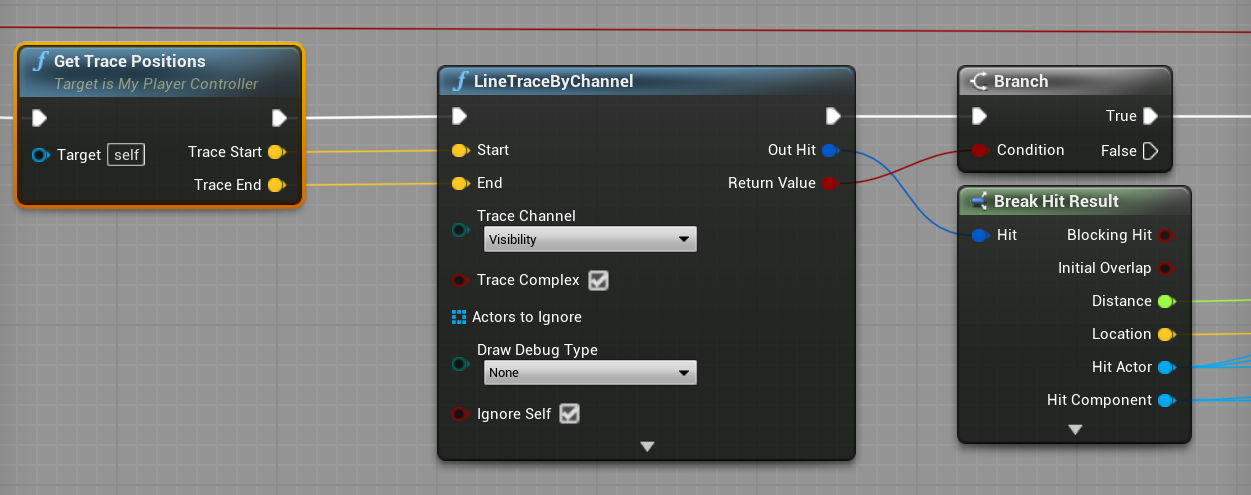
\includegraphics[width=0.8\textwidth]{fig/LineTracing.png}
	\caption[Tracing Grabs in Blueprints]{Tracing Grabs in Blueprints\protect}
	\label{fig:LineTracing}
\end{figure}
\subsection{Grabbing Individual Components}

As already mentioned, the model generally consists of many smaller components and while it is great to be able to interact with it as a whole, it could be a lot more useful if a user could choose to interact with every component individually.
%hovering

\subsection{Scaling and Rotating}

\subsection{Duplication, Expansion and Deletion}




\newpage
\newpage\thispagestyle{empty}\hspace{1em}\newpage
\chapter{Results and Evaluation}\label{chp:Results}

\section{CAD Runtime Importer and Presenter}

The projects described in Chapter \ref{chp:ObjectLoading} are called CAD Runtime Importer (\acs{CRI}) and CAD Runtime Presenter (\acs{CRP}). Both of these project's current release versions and source code of the whole project can for now be found on GitHub \url{https://github.com/MatijaMi/CADRuntime}. In the repository there are also instructions for using both programs. Depending on how and if Inosoft wants to use this project, there is a chance of that changing.\\
The plug-in itself contains all the code needed for opening, parsing and generating CAD models as well as the CRIObject class and the two required materials. In order to use it, the content of the ZIP file needs to be extracted into the plug-ins folder of the project and then the project just needs to be compiled once in order to register it. Once that is done, the CRIObject can be spawned, given the appropriate files and the generating will begin on its own. The plug-in can also easily be extended or adjusted for the concrete case it is being used for. Currently it can be used in Unreal Engine 4 versions 4.23 and higher. Unreal Engine 5 isn't supported but the changes introduced with it shouldn't influence the plug-in much so porting should be possible.\\
The presenter is a standalone program which can be used to load and interact with runtime generated objects in a multi-user environment. It offers its own file picker, as well as the option of sharing remote files through links. It enables all the interactions described in Chapter \ref{chp:ObjectInteraction}. It has two releases, the desktop and VR version that can be launched through their respective executables. There were ideas of trying to combine these two into one but generally this isn't done. The standard way of doing this is by having two separate versions. The VR version is fully compatible with the Oculus Quest 1 and 2 headsets. Other headsets could be supported through small adjustments but as they weren't available, this could not be achieved. For networking a session-based setup using the Steam online subsystem API was used. This means that a user hosts a section, acting as a listen server, while other users can join the session through a session browser. The connection between the users and listen server itself is handled through Steam. This was also tested with a total of four users at the same time and it worked without any major problems. One important feature that was needed in order for this to work is automatic mesh generation on joining a session. As the runtime generated meshes are not part of the level, they also do not get loaded for a new user when they connect to the session. That's why, when a new user joins, the program automatically downloads and generates all the existing meshes, including standalone Components. All of the meshes are also properly translated, scaled and rotated in order to match the state found on the server. 

\section{Performance and Comparison to Related Works}

In order to evaluate the plug-in's performance, it was compared to the two best options currently available, Datasmith Runtime and glTFRuntime. Datasmith Runtime, as mentioned before, is Unreal's official plug-in for CAD runtime importing. It is still quite new, as it was released in August 2021 and is still in beta\cite{bib:DSRunDoc}. On the other hand, glTFRuntime is an unofficial plug-in that has been in development for around two years and focuses purely on the import of glTF files\cite{bib:glTFRun}.\\
In order to truly test these programs, it was decided to use a rather large model, containing around 3 million vertices and 6 million faces. Tests with smaller objects were also done but they didn't have enough of an impact on any of the options to create meaningful results. First it was tested how long it took each plug-in to load in the model, in order to compare the speeds of the generating approaches. Then the frame rate of the project was tested to see how well it performed with one of these objects loaded in. This was then also repeated with multiple copies of the same object to see if the way the meshes were generated caused any differences. As a baseline for this, the same tests were done but with the model being added to the editor through regular Datasmith and placed in the scene before runtime. This way, it can be seen how much of the performance is simply caused by Unreal and how much by the runtime generation. All of these tests were run in the same Unreal project on a computer using a Ryzen 5 1500x processor, RX 470 graphics card and 16 gigabytes of RAM. This is definitely not the strongest machine but that should make it easier to see how well optimized the solutions are. The only difference between the tests is the file format used for them. For \acs{CRI} an OBJ file was used, while for the rest this OBJ was converted to glTF. The conversion was done with multiple programs and the best performing file was chosen. This was done in order to mitigate possible inefficiencies caused by converters. The OBJ and glTF files do contain the same number of vertices and faces so it shouldn't cause too much of a problem, perhaps only when it comes to parsing the files. The results of the loading time tests can be seen in Table \ref{tab:TimeResults}, where the values show the average time across 5 loads. For the performance test, Table \ref{tab:TimeResults} shows the average frames per second after a certain amount of copies of the large object were created with each program.\\


\begin{table}[htbp]
	\centering 
	\scalebox{0.889}{
		\begin{tabular}{|l|c|}
			\hline
			\textbf{Program} & \textbf{Time (s)}\\
			\hline
			Editor & 150,11\\
			\hline
			Datasmith & 131,62 \\
			\hline
			CRI & 35,48 \\
			\hline
			glTFRuntime & 41,37 \\
			\hline
	\end{tabular}}
	\caption[Time needed to generate object from file in seconds]{Time needed to generate object from file in seconds}
	\label{tab:TimeResults}
\end{table}

\begin{table}[htbp]
	\centering 
	\scalebox{0.889}{
		\begin{tabular}{|l|c|c|c|c|c|}
			\hline
			 \textbf{Program} & \textbf{1 Model} & \textbf{2 Models} & \textbf{3 Models} & \textbf{4 Models} & \textbf{5 Models} \\
			\hline
			Editor & 88 & 59 & 39  & 30  & 25 \\
			 \hline
			Datasmith & 76 & 48 & 33  & 22  & 17\\
			 \hline
			 CRI & 75 & 50 & 35  & 28  & 23 \\
			 \hline
			glTFRuntime & 54 &  30 & 21 & 17  & 7 \\
			 \hline
	\end{tabular}}
	\caption[Average frame rate per number of loaded Models]{Average frame rate per number of loaded Models}
	\label{tab:TestResults}
\end{table}

While the times show that \acs{CRI} is technically the fastest there are some things that need to be considered. First of all, loading in the file to the editor is a slightly different operation than just loading a mesh. It needs to create the appropriate assets and files so that Unreal can effectively work with this new object. Also, once that is done, adding the new object to a scene can be done multiple times and very quickly. Something quite similar can also be seen with Datasmith. The loading also takes quite long, probably because the internal workings are quite similar. This can be further seen when trying to load the same file again because the new instances appear within seconds. Compared to that, CRI times for creating a copy are always at least what is seen in the table, if not worse once the program becomes quite resource heavy. This is definitely an optimization on Datasmith's part but it's not quite clear if it just copies the object or has some sort of asset which is used to create new instances. This is mostly speculation but it would explain why these two have such similar times and make sense considering they are part of the same software.\\
Lastly it can be seen that \acs{CRI} is slightly faster than glTFRuntime but not by much. The difference could be due to the different file formats. This does at least prove that the times for Datasmith and the Editor aren't high only due to the format but because of what is happening under the hood. So overall \acs{CRI} is definitely fast enough but would be slightly worse than some when it comes to creating multiple instances.\\

When it comes to performance once the models are loaded in, it is clear that doing it in runtime has a noticeable performance impact. One of the reasons for this could definitely be increased RAM usage which was seen when creating meshes in runtime. It varied quite a bit from run to run but was consistently higher than when the models were part of the scene. Out of all the options, glTFRuntime fared the worst. It isn't quite clear why, but it probably has something to do with the way their meshes are generated. It is still an incredible tool that has many interesting features tuned to glTF files, it just doesn't handle many vertices as well. On the other hand, CRI and Datasmith are within margin of error between each other. Further tests were done with different files but this behaviour stayed the same. CRI does interestingly handle multiple objects ever so slightly better but at that point the frame rate isn't really usable any more. It is nonetheless impressive that Unreal and these plug-ins can handle more than 15 million vertices and 30 million faces created during runtime without crashing. 

\section{Shortcomings and Possible Improvements}

Overall, the biggest drawback for the plug-in are definitely the supported formats. While OBJ and STL allow it to support many formats indirectly, their properties do limit some features, such as scale and \acs{PBR} materials, from being completely realized. In order to fix this more parsers for more formats would need to be written. This isn't generally too difficult to do as long as the formats are well documented, but it can take some time to write a good, efficient parser. Unfortunately, there just wasn't enough time for that, as a lot of time went into learning and understanding how Unreal Engine works. Similarly, quite a bit of time was spent experimenting with different approaches for achieving the best results that could viably be implemented. This is also partly the reason why currently textures aren't supported. The main reasons were the fact that a lot of \acs{CAD} formats omit that information and that there are already proven ways of doing this in runtime\cite{bib:RunTex}. If development of this plug-in were to continue, these are definitely the features that would be added first.\\
When it comes to the presenter, the biggest problem is the reliance on the Steam online subsystem. While it is incredibly handy for small projects and experimenting, for the areas where this would potentially be used this isn't adequate. Ideally a dedicated server should be used as it wouldn't have to graphically render the newly generated objects causing less strain on it and the connected users. But creating such a server is very tedious as it means the project would have to be written in the source version of Unreal Engine. For that the whole source code of Unreal has to be downloaded and built which can easily take up more than 150 gigabytes of hard disk space. And that is just for the ability to make a project which can be packaged as a server.\\ 
Another problem that could arise can be found in file sharing. With small files the current approach works quite well but that is not the case with big files. Having to download quite large files can simply take a while and that definitely makes the user-experience a lot worse. Instead, if the files were available locally to every client and there was a way for every client to find the it once it was chosen by a different user, there wouldn't have to be any waiting. This would require a bit of preparation beforehand but it would still be better than having to share new versions of a program in order to add objects.\\
\newpage
\newpage\thispagestyle{empty}\hspace{1em}\newpage
\chapter{Conclusion}\label{chp:Conclusion}

Unreal Engine is an incredibly interesting and very unique piece of software with all of its features and functionalities. It is no surprise that it is seeing so much interest from various industries outside of game development. It is also no surprise that Unreal has to adapt in order to better suit these brand-new use-cases which bring with them completely new demands.\\
One example of that, the dynamic insertion of 3D objects from external CAD files, was demonstrated in this project. It is something that in traditional game development would make little to no sense. Considering the results of the performance test seen in Chapter \ref{chp:Results}, it is quite clear why this is the case. Nevertheless, it also cannot be denied that there is a certain demand for such a feature and that Unreal does have the means for it in its system. The only real problem is somehow getting access to it.\\
One way to realize this was used for the development of the \acs{CRI} plug-in. While it is slightly unfortunate that a separate plug-in had to be used, Runtime Mesh Component is brilliant and without it the achieved results probably would not have been possible in the limited amount of time available for this project. Notably one of the main goals of the project, which is efficiency. At its current state, when it comes purely to generating vertices and faces, the performance is even better than expected, being comparable to the official solution from Epic Games. Of course, it needs to be repeated that Datasmith Runtime is still in beta and that it is probably going to get better as development continues. It would especially be interesting to see just how close the performance of runtime generated objects can get to normally generated ones. It is feasible that some amount of changes to the low-level systems of Unreal could be necessary to achieve that.\\
The other goal of the plug-in, expandability, was also achieved. With the documentation in the repository and in the source code, it should be quite simple to adjust and widen the capabilities of it. Unfortunately, this is undeniably needed as there are still some limitations to functionalities caused by the lack of time that was available to be spent on them.\\
The area where runtime generation will probably see the most adoption is in projects like CAD Runtime Presenter. Being able to quickly load in a new model and simply present it to many users in VR can be quite handy. \acs{CRP} also already showed some of the things that can be done with interaction, but that is without a doubt just a small fraction of the possibilities. It is conceivable that not only presentation but also designing and creating new models could be done during runtime with multiple users. Creating a selection of simpler shapes that can be adjusted and attached to each other in different ways should definitely be possible. With dynamic materials instances, the materials could easily be changed and adapted as that only requires changing some values. This does raise a question in the opposite direction of this project. Would it be possible to generate completely new models in runtime and then somehow save them to actual CAD formats? Would perhaps a new format be necessary? Also, for models that were loaded in from external files, would there be a way to save changes made to it in runtime directly to the original file?\\
All in all, this a very interesting topic and there are definitely countless more projects, both official and unofficial, that will be made to further expand what is possible with Unreal Engine. Maybe it will come full circle and some creative developer will find a use for it in game development.

\newpage

\nocite{*}%Auch nicht-zitierte BibTeX-Einträge werden angezeigt.
\bibliography{Literaturverzeichnis}
\bibliographystyle{eg-alpha}
\newpage
\newpage\thispagestyle{empty}\hspace{1em}\newpage
\chapter*{List of Abbreviations}
\begin{acronym}[PM]
 %Sorgt dafür, dass zwischen den Einträgen kein Abstand ist und das Verzeichnis kompakt dargestellt wird.
 \setlength{\itemsep}{-\parsep}
 \acro{CAD}{Computer-aided design}
 \acro{VR}{Virtual reality}
  \acro{glTF}{Graphics Language Transmission Format}
  \acro{FBX}{Filmbox}
  \acro{AI}{Artificial Intelligence}
  \acro{API}{Application Programming Interface }
  \acro{RPC}{Remote Procedure Call}
  \acro{CRI}{CADRuntimeImporter}
  \acro{CRP}{CADRuntimePresenter}
  \acro{HTTP}{Hypertext Transfer Protocol}
  \acro{MTL}{Material Template Library}
  \acro{PMC}{Procedural Mesh Component} 
  \acro{RMC}{Runtime Mesh Component}
  \acro{PBR}{Physically Based Rendering}
\end{acronym}

%Abkürzungsverzeichnis im Inhaltsverzeichnis anzeigen
\addcontentsline{toc}{chapter}{List of Abbreviations} 
%Abbildungsverzeichnis
\newpage\thispagestyle{empty}\hspace{1em}\newpage
\listoffigures
%Tabellenverzeichnis
\listoftables
%Liste von Algorithmen
\newpage\thispagestyle{empty}\hspace{1em}\newpage
\markboth{List of Algorithms}{List of Algorithms}
\phantomsection
\addcontentsline{toc}{chapter}{List of Algorithms}
\listofalgorithms
%Liste von Code
\newpage\thispagestyle{empty}\hspace{1em}\newpage
\markboth{Listings}{Listings}
\phantomsection
\addcontentsline{toc}{chapter}{Listings}
\lstlistoflistings

\end{document} 